\chapter{问题分析和框架设计}
\label{cha:problem_framework}

\section{本章引论}

随着互联网上不同类型的平台出现,人们每天在各种平台上产生着各种各样的行为和发言。如现在微博平台上会对热门时事设置井号标签,人们透过加上对应标签来表达对该事件的想法,以及透过对这些发言进行赞点、分享或评论来表达支持或反驳。透过根据井号标签收集数据并进行意图分析可以得知网民对该事件的舆论方向。在其他平台上的各种行为记录同样可能有挖掘其意图的价值,意图识别的应用场景也变得多种多样,但即使数据的内容和结构不同,问题的本质是相似的。因此在本章,我们将首先针对意图识别进行分析,并给出统一的形式化表示。

再进一步,基于该形式化表示,我们提出一个面向社交媒体文本的意图识别研究框架。从原始文本的输入到最终识别目标的输出,理清其中每个步骤的功能和目的,给出一个完整识別系统的实现流程,为解决后续章节中研究的问题准备一个统一的切入点。


\section{问题分析}

本小节中,我们将对意图识别中涉及的各个元素作出分析,并给出统一的形式化表示来描述他们的相互关系。

不同意图识别问题中都有要被识别的目标$C$。如Tang等人\cite{tang2015learning}的情感极性识别研究,$C$对应需要五级的情感极性。在刘丹丹等人\cite{刘丹丹2015基于}的微博情感分类研究中,$C$对应喜好、安乐、惊奇、厌恶、悲哀、愤恨、恐惧。邓钊等人\cite{2015面向微博的中文反语识别研究}的中文反语识别研究中,$C$则对应是否包含反讽。

其次是研究主体$T$,它是行为发起者$S$的行为记录,可以认为是其想法和情感的载体。如以讨论区上的帖子作为研究主体,那么$C$就是帖子的内容,包括其中的文本内容、图片、文件附件等,$T$则是帖子的发布者。另外一些场景下会有背景信息$B$,对应所有有助于正确理解$C$的信息,如帖子所在讨论区的类型有助于定位帖子对应的领域,发布者的发布历史显示发布者的一些态度倾向,帖子下的评论从侧表反映主帖的内容,这些都可能是理解帖子内容的提示。

意图识别假设对于任意一个研究样本$t \in T$,在给定背景信息$b \in B$(或其些情况下无需背景信息),其承载想法或情感必然存在对应的倾向$c \in C$。意图识別首先要从样本主体和背景信息中分別提取出识別目标相关的信息$f_t$和$f_b$,即需要提出两个映射函数,$F_T$和$F_B$,满足 $f_t=F_T(t)$和$f_b=F_B(b)$。再进一步根据相关信息识別出其想法或情感倾向,即找出一个映射$F_C$,使得 $c=F_C(f_t, f_b)=F_C(F_T(t), F_B(b))$。

\section{框架设计}

在本小节,我们将根据前述的形式化表示给出一个意图识别的研究框架。由于在本论文的后续研究均面向英语難金社交媒体文本的分类问题,我们会针对此研究方法对框架进行细化,从原始文本的输入到最终识别目标的输出,理清其中每个步骤的功能和目的,给出一个完整系统的实现流程。

\begin{figure}[H] % use float package if you want it here
  \centering
  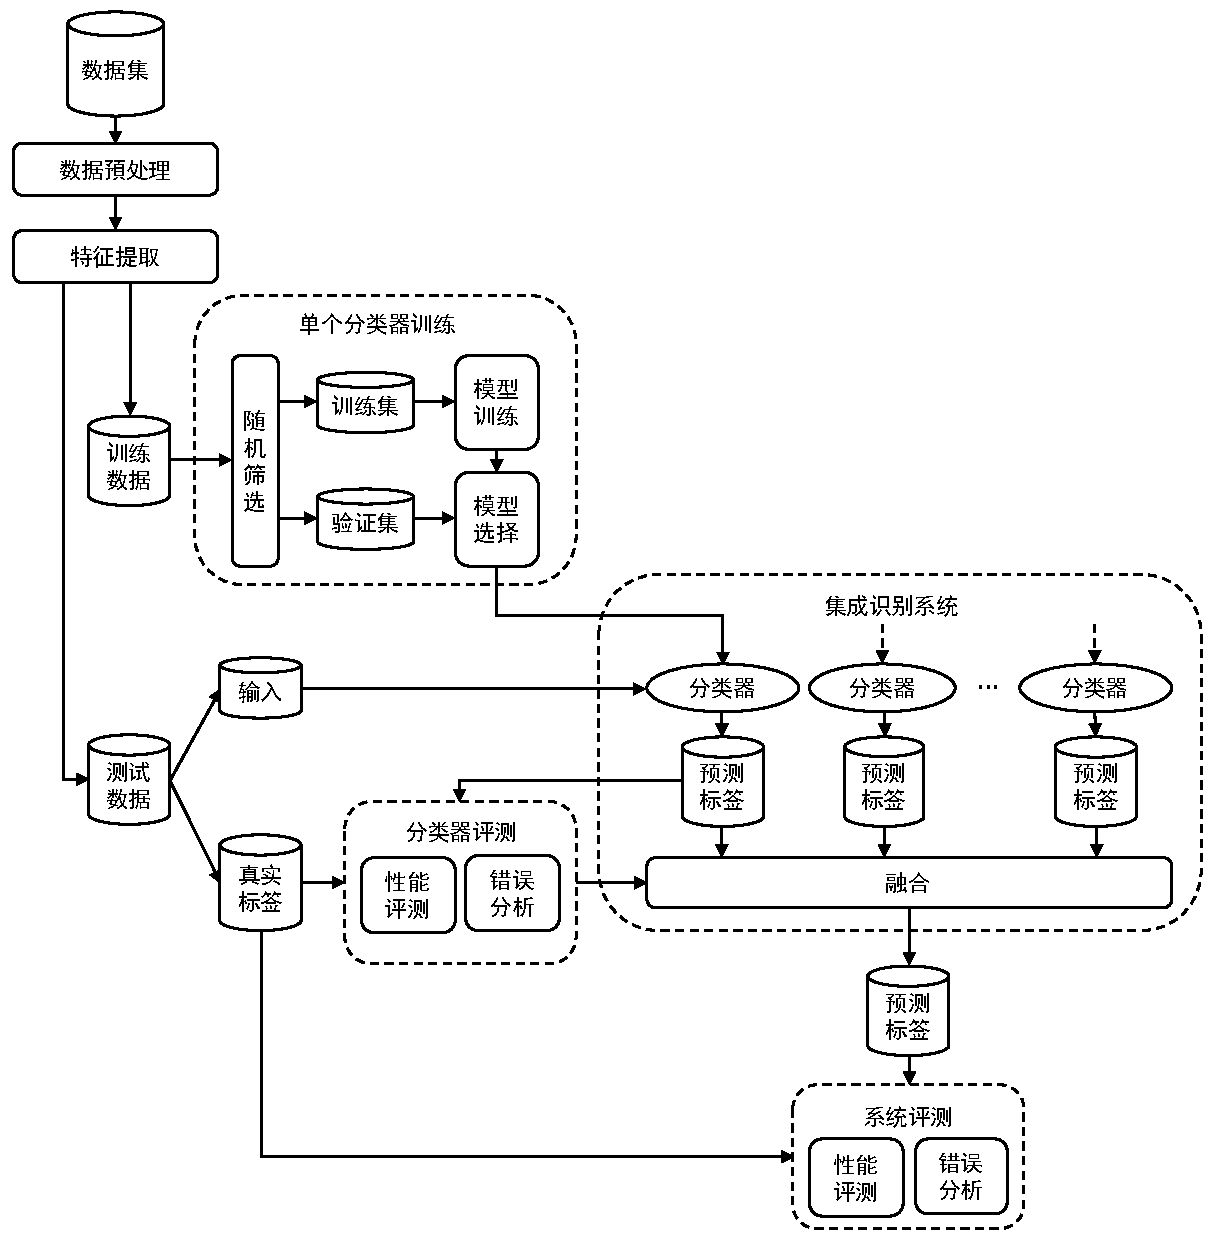
\includegraphics[width=\textwidth]{img/framework.pdf}
  \caption{意图识别的研究框架}
  \label{fig:framework}
\end{figure}


\section{本章小结}

pass

